\documentclass[float=false, crop=true]{standalone}
\usepackage{import}
\usepackage{tikz}
\usepackage{pgfplots}
\usetikzlibrary{calc}
\usetikzlibrary{arrows}

\begin{document}




\tikzset{every picture/.style={line width=0.75pt}} %set default line width to 0.75pt        

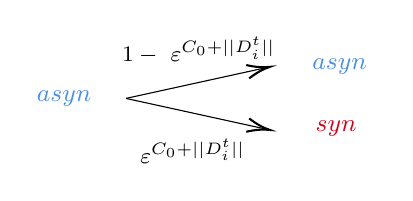
\begin{tikzpicture}[x=0.75pt,y=0.75pt,yscale=-1,xscale=1]
%uncomment if require: \path (0,273); %set diagram left start at 0, and has height of 273

%Straight Lines [id:da14332591914208104] 
\draw    (307.66,39.24) -- (375.02,24.46) ;
\draw [shift={(376.98,24.03)}, rotate = 167.63] [color={rgb, 255:red, 0; green, 0; blue, 0 }  ][line width=0.75]    (10.93,-3.29) .. controls (6.95,-1.4) and (3.31,-0.3) .. (0,0) .. controls (3.31,0.3) and (6.95,1.4) .. (10.93,3.29)   ;
%Straight Lines [id:da8559685352825592] 
\draw    (307.66,39.24) -- (375.02,54.01) ;
\draw [shift={(376.98,54.44)}, rotate = 192.37] [color={rgb, 255:red, 0; green, 0; blue, 0 }  ][line width=0.75]    (10.93,-3.29) .. controls (6.95,-1.4) and (3.31,-0.3) .. (0,0) .. controls (3.31,0.3) and (6.95,1.4) .. (10.93,3.29)   ;

% Text Node
\draw (279.9,39.12) node  [font=\small]  {$\textcolor[rgb]{0.29,0.56,0.89}{asyn} \ $};
% Text Node
\draw (412.62,23.91) node  [font=\small]  {$\textcolor[rgb]{0.29,0.56,0.89}{asyn} \ $};
% Text Node
\draw (408.87,53.82) node  [font=\small]  {$\textcolor[rgb]{0.82,0.01,0.11}{syn}$};
% Text Node
\draw (339.78,64.57) node  [font=\footnotesize]  {$\varepsilon ^{C_{0} +||D_{i}^{t} ||}$};
% Text Node
\draw (342.71,16.07) node  [font=\footnotesize]  {$1-\ \varepsilon ^{C_{0} +||D_{i}^{t} ||}$};


\end{tikzpicture}



\end{document}